\documentclass[titlepage]{article}
\usepackage[czech]{babel}
\usepackage{pdfpages}
\usepackage{amsmath}
\usepackage{pgfplots}
\usepackage{siunitx}
\usepackage[parfill]{parskip}
\usepackage{float}
\usepackage{hyperref}
\hypersetup{
    colorlinks,
    citecolor=black,
    filecolor=black,
    linkcolor=black,
    urlcolor=black
}
\sisetup{detect-all}

\begin{document}
%opening
\begin{titlepage}
 \includepdf{razitko.pdf}
\end{titlepage}

\tableofcontents
\newpage

\section{Úkol měření}

\begin{enumerate}
 \item Změřte závislost anodového proudu $I_A$ na napětí $U_G$ speciální elektronky ve Franckově - Hertzově pokusu při vybrané teplotě z intervalu $160  - 250 \si{\celsius}$. Závislost znázorněte graficky.

 \item Nalezněte všechna měřitelná minima této závislosti při dalších dvou teplotách z uvedeného intervalu.

 \item Z naměřených hodnot stanovte excitační energii atomu rtuti a příslušnou vlnovou délku emitovaného světla.
\end{enumerate}

\section{Seznam použitých přístrojů}
\begin{itemize}
\item Multimetr MY-65
 \begin{itemize}
  \item rozsah $200 \si{\volt}$, přesnost $\pm 0.1 \%$ z údaje $\pm 1$ digit
 \end{itemize}

\item Nanoampérmetr
 \begin{itemize}
  \item třída přesnosti 1.5
 \end{itemize}

\item pícka s elektronkami a mřížkou
\end{itemize}

\section{Teoretický úvod}
\subsection{Excitace atomů}
Excitovaný stav atomu je stav s vyšší energií než základní stav. Tedy musíme atomu energii dodat. V našem případě využijeme exciatci s původem ve srážce elektornu s atomem.

\subsection{Franckův-Hertzův pokus}
Pokusy spočívají v tom, že atomy plynu jsou odstřelovány pomalými elektrony. Při tomto odstřelování pozorujeme rozložení rychlostí elektronů před a po srážce.

Ke srážce elektronů a atomů dochazí v elektronkové triodě. Ta je naplněna parami rtuti. Žhavená katoda \textbf{K} uvolňuje termoemisí elektrony, které jsou urychleny mezi katodou a kladně nabitou mřížkou \textbf{G} a vstupují do experimentálního prostoru. V tomto prostoru se nachází anoda \textbf{A}. Mezi mřížkou a anodou se udržuje malý potenciálový rozdíl $U_B$, takže k proudu $I_A$ přispívají jen elektrony s energíí vyšší než jisté minimum energie. Se zvyšováním urychlovacího potenciálu $U_G$ dopadá na destičku větší počet elektronl a tudíž proud $I_A$ roste.

Rychlost $v$, kterou získavají elektrony vlivem napětí $U_G$ je dána vztahem
\begin{equation}
 \frac{1}{2} m v^2 = e U_G
\end{equation}
kde $m$ je hmotnost atomu a $e$ je jeho měrný náboj.

Z tohoto vzathu dostáváme dosazením konstant následující
\begin{equation}
 v = \sqrt{\frac{2 e U_G}{m}} \simeq 5.93 \cdot 10^5 \sqrt{U_G}\ \ \ [\si{\meter \per \second}]
\end{equation}

Po dosažení určité kinetické energie elektronů anodový proud $I_A$ klesá. Toto se dá vysvětlti tím, že elektron pozbyde svoji energii excitací atomu rtuti na evyšší energetickou hladinu. Toto se opakuje pro každou energetickou hladinu atomu.

\subsection{Výpočet excitční energie atomu}
Nechť potenciál kotody se rovná nule a potenciál anody je rove $+ \varphi_A$. Krotický potenciál, kdy nastane srážka je $\varphi_k$. SPád potenciálu $\varphi_A$ je po celé délce od K do A. Nechť elektron prodělá srážku v bodě s potenciálem $\varphi_x$. Po srážce bude tedy mít energii $e(\varphi_x - \varphi_k)$. Při dosažení elektrody A bude mít energii $E$ danou vztahem
\begin{equation}\label{eq:energy}
 E = e(\varphi_x - \varphi_k) + e(\varphi_A - \varphi_x) = e(\varphi_A - \varphi_k) = \Delta U_G
\end{equation}
Kde $\Delta U_G$ je rozdíl vzdáleností minim voltampérové charakteristiky.

Následný přechod do základního stavu je poté spojen s vyzářením fotonu s frekvencí $\nu$ která je dána vztahem
\begin{equation}\label{eq:freq}
 \nu h = E
\end{equation}
kde $h$ je Planckova konstanta.

Z této frekvence jsme následně schopni stanovit vlnovou délku vyzařovaného světla $\lambda$
\begin{equation}\label{eq:wave}
 \lambda = \frac{c}{\nu}
\end{equation}
kde $c$ je rychlost světla.

\newpage
\section{Naměřené hodnoty a jejich zpracování}
\subsection{Závislost anodového proudu $I_A$ na napětí $U_G$}
\subsubsection{Naměřené hodnoty}
Při měření jsme zapisovali údaj $N$ a rozsah $R$ nanoampérmetru.
\begin{table}[H]
    \begin{minipage}{.49 \textwidth}
      \centering
        \begin{tabular}{c||c|c|c|c}
            $t [\si{\celsius}]$ & $U_G [\si{\volt}]$ & $N$ & $R$ & $I_A [\si{\nano\ampere}]$ \\ \hline\hline
            169 & 4.29 & 90 & 0.2 & 0.18 \\ \hline
            166 & 4.87 & 75 & 1 & 0.75 \\ \hline
            168 & 6.09 & 90 & 2 & 1.80 \\ \hline
            171 & 6.82 & 45 & 1 & 0.45 \\ \hline
            172 & 7.91 & 30 & 0.2 & 0.06 \\ \hline
            170 & 8.75 & 55 & 1 & 0.55 \\ \hline
            168 & 10.83 & 70 & 20 & 14.00 \\ \hline
            171 & 12.18 & 50 & 1 & 0.50 \\ \hline
            171 & 13.05 & 30 & 0.5 & 0.15 \\ \hline
            169 & 13.86 & 50 & 5 & 2.50 \\ \hline
            169 & 15.82 & 55 & 50 & 27.50 \\ \hline
            170 & 16.99 & 50 & 10 & 5.00 \\ \hline
            171 & 17.85 & 70 & 2 & 1.40
        \end{tabular}
        \caption{Nastavená teplota $170\ \si{\celsius}$}
    \end{minipage}%
    \begin{minipage}{.49 \textwidth}
      \centering
        \begin{tabular}{c||c|c|c|c}
            $t [\si{\celsius}]$ & $U_G [\si{\volt}]$ & $N$ & $R$ & $I_A [\si{\nano\ampere}]$ \\ \hline\hline
            204 & 4.95 & 25 & 0.5 & 0.13 \\ \hline
            207 & 5.91 & 90 & 0.5 & 0.45 \\ \hline
            207 & 6.60 & 30 & 0.5 & 0.15 \\ \hline
            205 & 8.53 & 10 & 0.2 & 0.02 \\ \hline
            201 & 9.73 & 60 & 1 & 0.60 \\ \hline
            199 & 10.73 & 40 & 5 & 2.00 \\ \hline
            197 & 11.32 & 60 & 1 & 0.60 \\ \hline
            199 & 13.34 & 5 & 0.2 & 0.01 \\ \hline
            200 & 13.92 & 55 & 1 & 0.55 \\ \hline
            202 & 15.29 & 45 & 10 & 4.50 \\ \hline
            201 & 16.08 & 55 & 2 & 1.10 \\ \hline
            197 & 17.95 & 5 & 0.2 & 0.01 \\ \hline
            203 & 18.89 & 55 & 1 & 0.55 \\ \hline
            203 & 20.25 & 75 & 5 & 3.75 \\ \hline
            201 & 21.16 & 40 & 2 & 0.80 \\ \hline
            200 & 22.53 & 5 & 0.2 & 0.01 \\ \hline
            198 & 23.56 & 50 & 2 & 1.00 \\ \hline
            199 & 25.15 & 50 & 20 & 10.00
        \end{tabular}
        \caption{Nastavená teplota $200\ \si{\celsius}$}
    \end{minipage}
\end{table}
\begin{table}[H]
    \begin{minipage}{.49 \textwidth}
      \centering
        \begin{tabular}{c||c|c|c|c}
            $t [\si{\celsius}]$ & $U_G [\si{\volt}]$ & $N$ & $R$ & $I_A [\si{\nano\ampere}]$ \\ \hline\hline
            237 & 5.38 & 15 & 0.2 & 0.03 \\ \hline
            236 & 6.25 & 45 & 0.2 & 0.09 \\ \hline
            233 & 7.79 & 25 & 0.2 & 0.05 \\ \hline
            231 & 8.20 & 15 & 0.2 & 0.03 \\ \hline
            230 & 8.67 & 10 & 0.2 & 0.02 \\ \hline
            230 & 9.13 & 10 & 0.2 & 0.02 \\ \hline
            224 & 9.36 & 15 & 0.2 & 0.03 \\ \hline
            232 & 10.19 & 30 & 0.5 & 0.15 \\ \hline
            230 & 10.83 & 35 & 1 & 0.35 \\ \hline
            232 & 11.51 & 45 & 0.5 & 0.23 \\ \hline
            231 & 13.17 & 15 & 0.2 & 0.03 \\ \hline
            231 & 13.40 & 10 & 0.2 & 0.02 \\ \hline
            230 & 13.75 & 5 & 0.2 & 0.01 \\ \hline
            230 & 14.08 & 10 & 0.2 & 0.02 \\ \hline
            230 & 15.16 & 45 & 0.5 & 0.23 \\ \hline
            231 & 15.91 & 50 & 1 & 0.50 \\ \hline
            233 & 16.87 & 40 & 0.5 & 0.20 \\ \hline
            231 & 17.77 & 10 & 0.2 & 0.02 \\ \hline
            231 & 18.07 & 5 & 0.2 & 0.01 \\ \hline
            230 & 18.43 & 5 & 0.2 & 0.01 \\ \hline
            229 & 18.50 & 10 & 0.2 & 0.02 \\ \hline
            229 & 19.72 & 50 & 1 & 0.50 \\ \hline
            232 & 20.36 & 50 & 2 & 1.00 \\ \hline
            233 & 21.58 & 30 & 0.5 & 0.15 \\ \hline
            232 & 22.35 & 10 & 0.2 & 0.02 \\ \hline
            231 & 22.45 & 5 & 0.2 & 0.01 \\ \hline
            \vdots & \vdots & \vdots & \vdots & \vdots
        \end{tabular}
    \end{minipage}%
    \begin{minipage}{.49 \textwidth}
      \centering
        \begin{tabular}{c||c|c|c|c}
            $t [\si{\celsius}]$ & $U_G [\si{\volt}]$ & $N$ & $R$ & $I_A [\si{\nano\ampere}]$ \\ \hline\hline
            \vdots & \vdots & \vdots & \vdots & \vdots \\ \hline
            229 & 22.67 & 5 & 0.2 & 0.01 \\ \hline
        228 & 23.10 & 10 & 0.2 & 0.02 \\ \hline
        227 & 24.06 & 40 & 1 & 0.40 \\ \hline
        232 & 25.35 & 75 & 2 & 1.50 \\ \hline
        232 & 26.04 & 45 & 1 & 0.45 \\ \hline
        230 & 26.99 & 10 & 0.2 & 0.02 \\ \hline
        230 & 27.23 & 5 & 0.2 & 0.01 \\ \hline
        230 & 27.71 & 5 & 0.2 & 0.01 \\ \hline
        229 & 27.80 & 10 & 0.2 & 0.02 \\ \hline
        230 & 28.69 & 45 & 1 & 0.45 \\ \hline
        230 & 30.44 & 40 & 5 & 2.00 \\ \hline
        227 & 30.92 & 50 & 1 & 0.50 \\ \hline
        227 & 31.92 & 10 & 0.2 & 0.02 \\ \hline
        231 & 32.30 & 5 & 0.2 & 0.01 \\ \hline
        233 & 32.63 & 5 & 0.2 & 0.01 \\ \hline
        235 & 32.67 & 10 & 0.2 & 0.02 \\ \hline
        230 & 33.78 & 55 & 1 & 0.55 \\ \hline
        227 & 34.99 & 45 & 5 & 2.25 \\ \hline
        230 & 35.92 & 40 & 1 & 0.40 \\ \hline
        232 & 36.88 & 10 & 0.2 & 0.02 \\ \hline
        232 & 37.26 & 5 & 0.2 & 0.01 \\ \hline
        231 & 37.38 & 10 & 0.2 & 0.02 \\ \hline
        230 & 37.45 & 15 & 0.2 & 0.03 \\ \hline
        229 & 38.56 & 50 & 2 & 1.00 \\ \hline
        229 & 39.85 & 70 & 5 & 3.50 \\ \hline
        229 & 40.67 & 50 & 2 & 1.00
        \end{tabular}
    \end{minipage}
    \caption{Nastavená teplota $230\ \si{\celsius}$}
\end{table}

\subsubsection{Graf závislosti anodového proudu $I_A$ na napětí $U_G$}

\begin{figure}[H]
    \centering
    \begin{tikzpicture}
        \begin{axis}[
            xlabel={$U_G [\si{\volt}]$},
            ylabel={$I_A [\si{\nano\ampere}]$},
        ]

        \addplot[color = blue]
            table[x=U,y=I,col sep=comma]{data/170deg.csv};
            \addlegendentry{$170\ [\si{\celsius}]$}

        \addplot[color = green]
            table[x=U,y=I,col sep=comma]{data/200deg.csv};
            \addlegendentry{$200\ [\si{\celsius}]$}

        \addplot[color = red]
            table[x=U,y=I,col sep=comma]{data/230deg.csv};
            \addlegendentry{$230\ [\si{\celsius}]$}
        \end{axis}
    \end{tikzpicture}
\end{figure}

\subsection{Výpočet energie atomů rtuti}
\subsubsection{Nalezená minima}
\begin{table}[H]
    \centering
    \begin{tabular}{c||c|c|c}
        ~ & \multicolumn{3}{c}{$min_i {U_G}\ [\si{e\volt}]$} \\ \hline
        i & $170\ \si{\celsius}$ & $200\ \si{\celsius}$ & $230\ \si{\celsius}$ \\ \hline\hline
        1 & 7.91 & 8.53 & 8.84 \\ \hline
        2 & 13.05 & 13.34 & 13.60 \\ \hline
        3 & 17.85 & 17.95 & 18.19 \\ \hline
        4 & ~ & 22.53 & 22.64 \\ \hline
        5 & ~ & ~ & 27.43 \\ \hline
        6 & ~ & ~ & 32.38 \\ \hline
        7 & ~ & ~ & 37.24
    \end{tabular}
\end{table}

\subsubsection{Výpočet energie}
Proložením metodou nejmenších čtverců s využitím principu postupné metody dostáváme $\Delta U_G = 4.7143\ \si{e\volt}$ a $\sigma_{\Delta U_G} =  0.035\ \si{e\volt}$. Za využití vztahu \eqref{eq:energy} pak dostáváme $E = \Delta U_G = 4.7143\ \si{e\volt}$.

\subsubsection{Výpočet vlnové délky vyzářeného atomu}
Dle vytahu \eqref{eq:freq} dostáváme frekvency
$$
\nu = \frac{E}{h} = \frac{4.7143\ \si{e\volt}}{4.135667 \cdot 10^{-15}\ \si{e\volt\per\hertz}}=1139.91\ \si{\tera\hertz}
$$.

Z té poté podle vytahu \eqref{eq:wave} dostáváme vlnovou délku
$$
\lambda = \frac{c}{\nu} = \frac{299792458\ \si{\meter\per\second}}{1139.91\ \si{\tera\hertz}} = 2.63 \cdot 10^{-7}\ \si{\meter} = 263\ \si{\nano\meter}
$$
\subsubsection{Výpočet nejistot}

\begin{gather*}
 u(\nu) = \sqrt{(\frac{ \partial \nu}{\partial E}u(E))^2} = \frac{u(E)}{h} = 8.46 \cdot 10^{12}\ \si{\hertz} = 8.46\ \si{\tera\hertz}\\
 \\
u(\lambda) = \sqrt{(\frac{ \partial \lambda}{\partial \nu}u(\nu))^2} = \frac{c}{\nu ^ 2}u(\nu) = 1.952 \cdot 10^{-9}\ \si{\meter} = 1.952\ \si{\nano\meter}
\end{gather*}

\section{Závěr}
Závislost anodového proudu $I_A$ na napětí $U_G$ a následně jsme z ní spočítali proložením excitační energii atomu rtuti $E = (4.714 \pm 0.035)\  \si{e\volt}$ a vlnovou délku vyzářeného světla po návratu do základního stavu $\lambda = (263.0 \pm 2.0)\ \si{\nano\meter}$. Tabulková hodnota excitační energie je $4.9\ \si{e\volt}$ od které se spočtená odlišuje o $3.8\%$ a tabulková hodnota vlnové délky je $\lambda = 253.6\ \si{\nano\meter}$ od které se ta spočtená odlišuje o $3.7\%$.

\section{Použitá literatura}
[1] Franckův-Hertzův pokus a stanovení excitační energie atomu rtuti [online] dostupné z: \\\url{planck.fel.cvut.cz/praktikum/downloads/navody/franckhertz.pdf}

\section{Přílohy}
\begin{figure}[H]
 \centering
 \begin{minipage}{0.4\textwidth}
  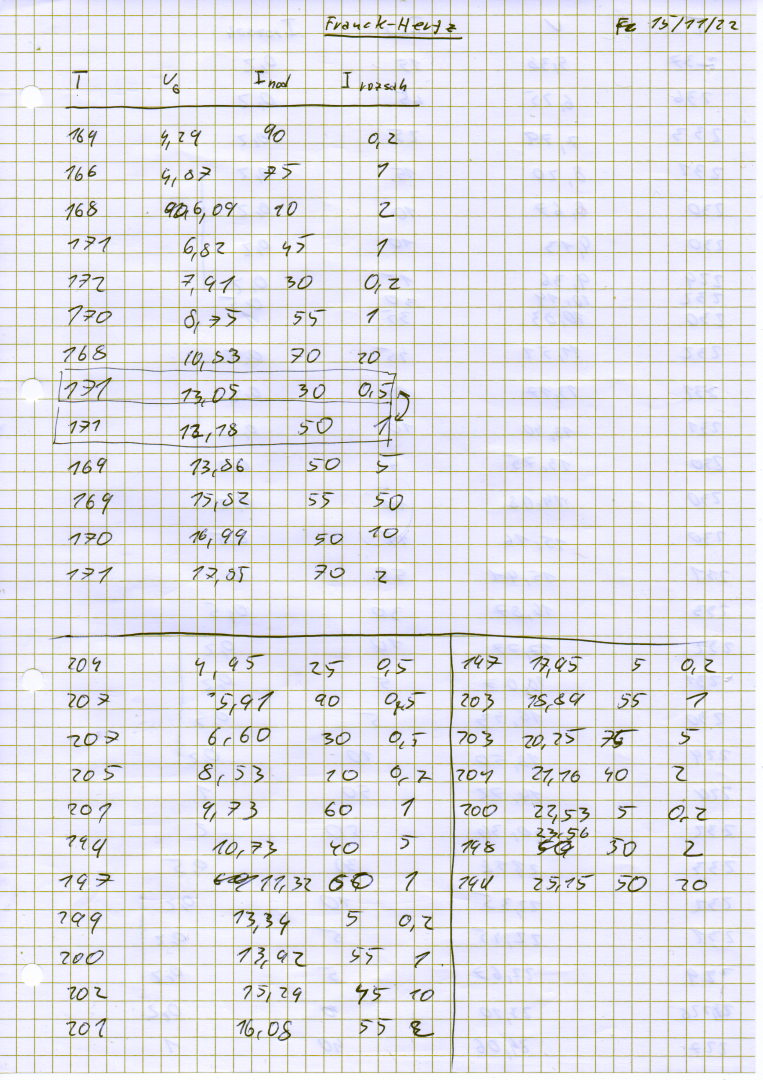
\includegraphics[width=\textwidth]{scan/page1.png}
 \end{minipage}
 \hfil
 \begin{minipage}{0.4\textwidth}
  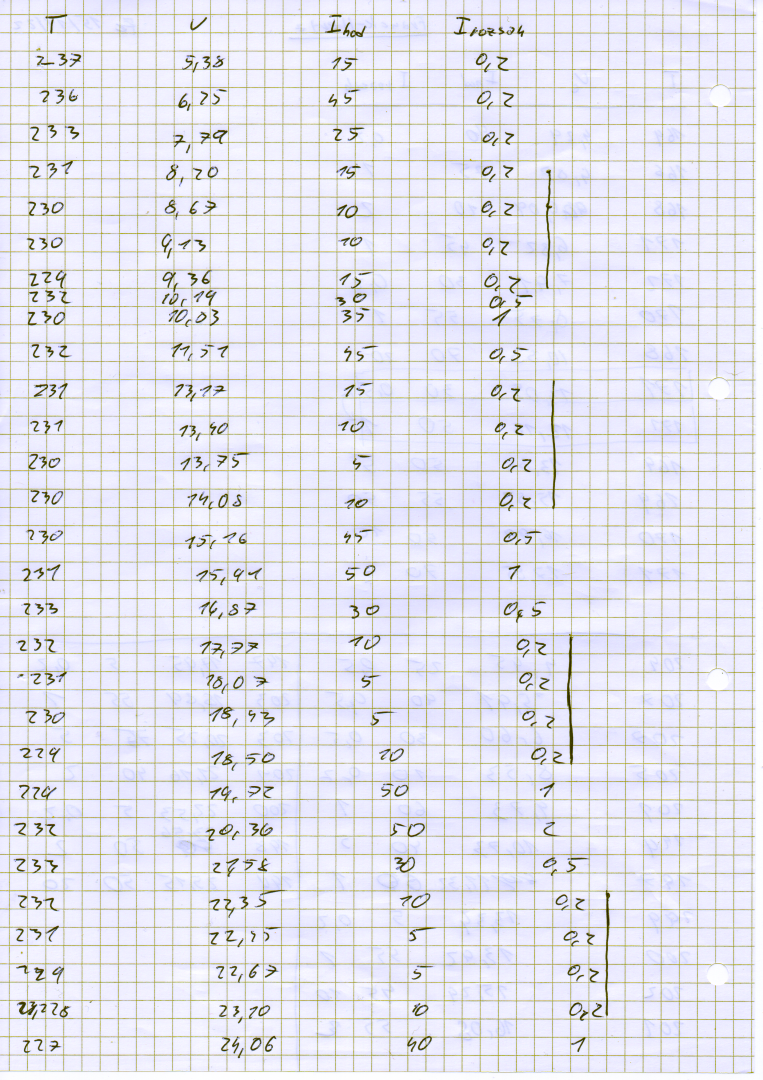
\includegraphics[width=\textwidth]{scan/page2.png}
 \end{minipage}
 \begin{minipage}{0.4\textwidth}
  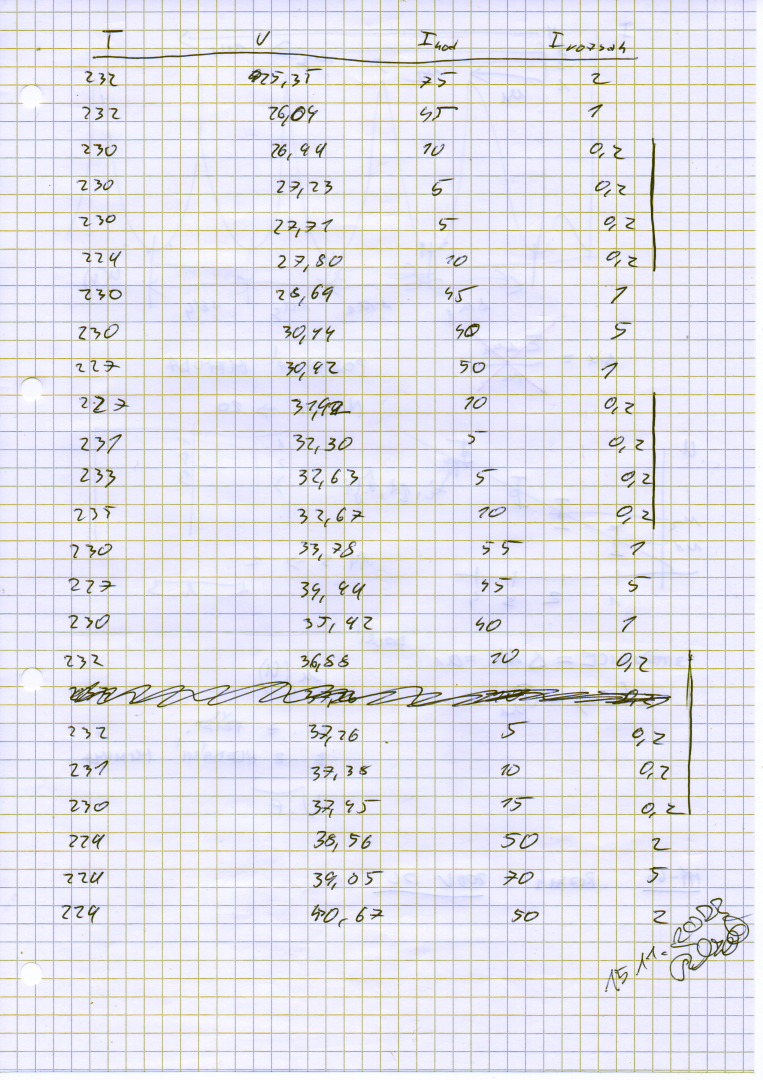
\includegraphics[width=\textwidth]{scan/page3.png}
 \end{minipage}
 \caption{Originální zápis naměřených hodnot}
\end{figure}

\end{document}
